\documentclass[a4paper]{article}

\usepackage[]{caption}
\usepackage[]{graphicx}
\usepackage[style=apa]{biblatex}
\usepackage[]{microtype}
\usepackage[table]{xcolor}
\usepackage[toc,page]{appendix}
\usepackage[margin=1.3in]{geometry}
\usepackage[]{sectsty}
\usepackage[]{setspace}
\usepackage[]{latexsym}
\usepackage[]{ragged2e}
\usepackage[colorlinks=true,citecolor=blue,linkcolor=blue]{hyperref}
\usepackage[capitalise]{cleveref}

\captionsetup[figure]{
  font = it,
  labelfont = bf
}

\graphicspath{{./graphs/}{./images/}}
\addbibresource{written-report.bib}

\begin{document}
\begin{titlepage}
  \Centering{}
  \Large{SINGAPORE-CAMBRIDGE GENERAL CERTIFICATE OF EDUCATION (H1) EXAMINATION} \\

  \vspace{1cm}

  \centering{\Large{PROJECT WORK}} \\

  
\includegraphics[scale=0.5]{ri-school-crest.png} \\
  \begin{tabular}{l@{:\hspace{1cm}}l}
    School & Raffles Institution \\
    Group number & RI013 \\
    Project task & 2
  \end{tabular} \\

  \vspace{2cm}

  \Huge{\textbf{Online scams in youths}} \\


  \vspace{2cm}

  \Large{
    \begin{tabular}{c c}
      \textbf{Candidate name} & \textbf{Candidate number} \\
      Alicia Chan Wen Yan & 30151154 \\
      Karthik Chidambaram & 30151160 \\
      Lyu Junwei & 30151164 \\
      Vera Tay Xiang Yu & 30151172 \\
      Yeo Jie Xuan, Isaac & 30151175
    \end{tabular} \\

    \vspace*{\fill}

    \small{\emph{Word Count: \ldots}} \\
  }
\end{titlepage}

\newpage

\pagenumbering{Roman}

\begin{abstract}
  \addcontentsline{toc}{section}{Abstract}
  \noindent
  \ldots?
\end{abstract}

\newpage


\tableofcontents

\newpage

\pagenumbering{arabic}

\section{Identification of problem}
\subsection{Choice of topic}
\paragraph{} As the world undergoes digitalisation, there has been a massive
uptick in the number of youths\footnote{In Singapore, youths are defined as
  people aged 15--35.} falling for scams in Singapore. This paper will address
the factors contributing to increased scam rates among youths and potential
solutions to stem the problem.

\subsection{Rationale for choice of topic}
Many day-to-day processes are shifting online, from e-commerce
\parencite{ITA.2022} to banking services \parencite{Degenhard.2023}.
Consequently, youths are spending more time on the Internet and falling for
online scams. The number of young people falling for online scams has grown from
15455 total cases in 2021 to a total of 23565 in 2022---more than a 50\% increase
\parencite{Tham.2023}. Moreover, it is extremely difficult for the police to
recover the money from scammers: in 2021, more than 90\% of scams originated
from overseas; hence, the monetary losses are largely irreversible
\parencite{Begum.2022}. This undermines Digital Defence, one of the pillars of
Singapore’s Total Defence \parencite{SCDF.2023}, implying Singapore’s security
is compromised.

\subsection{Significance of problem}
\paragraph{} On the individual level, scam victims tend to feel shame and
helplessness after getting scammed \parencite{CNA.2022}, putting them at
heightened risk of mental health issues \parencite{SiowDivi.2023}.

\paragraph{} Victims might also think that taking advantage of others’ trust is
commonplace. Thus, they may start losing trust in humans, becoming paranoid and
keeping to themselves if they normalise scammers’ dishonest behaviour
\parencite{SiowDivi.2023}. This may result in a widespread eradication of
once-strong interpersonal relationships.

\paragraph{} To society at large, the substantial amount of money lost to scams
in recent years suggests that falling for online scams has a large economic
impact on Singapore; the money lost to online scams has increased to almost
S\$1.3 billion from 2021 to 2022 \parencite{Chua.2023}.

\paragraph{}
Victims' vulnerability to the numerous scam opportunities implies an overall
decrease in the safety of online platforms, with a possible eradication of trust
in online processes. This compromises the reliability of online services like
banking and e-commerce as a whole, which preventing us from taking full
advantage of the benefits digitalisation has to offer. On a global scale
Globally, this also endangers Singapore’s reputation as a financial hub that
gives foreigners ``a strong sense of security and comfort'' \parencite{Rikvin}.

\subsection{Rationale for choice of target group}
\paragraph{} Our Target Group is youths aged 20--29.

\paragraph{} As most youth have just started working, there is understandably a
heightened want and need for money (\cref{fig:incomegraph}), making scam offers
seem attractive. However, this leaves them highly susceptible to scams: more
than 26\% of scam victims are 20--29 years old \parencite{Chua.2023}, comprising
the largest share of 2022 scam victims. As they ``lack the experience to deal
with complex issues'' \parencite{SiowDivi.2023}, they might not be able to cope
emotionally with the consequences of falling for a scam and their mental health
might be especially adversely affected.

\begin{figure}[ht]
  \centering 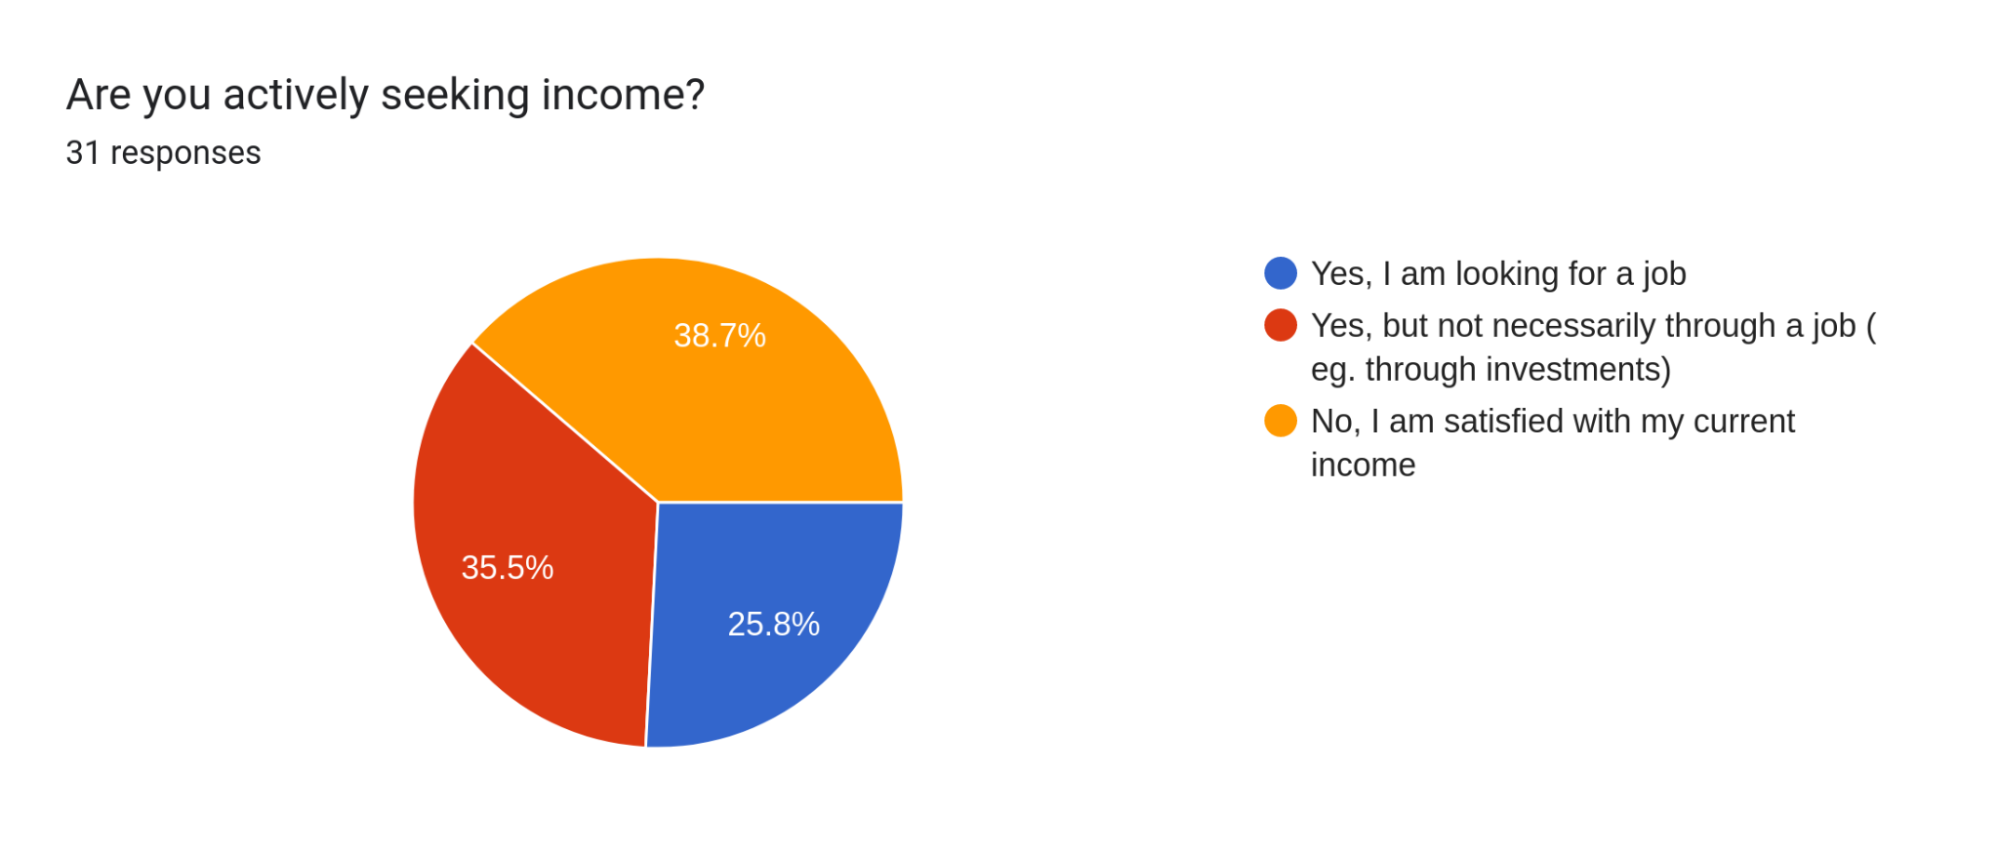
\includegraphics[width=\textwidth]{incomegraph}
  \caption{Chart from our survey of 31 respondents showing that more than half
    of the youth we surveyed are actively seeking income and hence display a
    want/need for money.}\label{fig:incomegraph}
\end{figure}

\paragraph{} Since youths are just entering the workforce and earn relatively
lower salaries, losses from scams may comprise a higher proportion of their
income, resulting in a greater threat to their ability to recover from the
financial blow.

\paragraph{} Considering that this group will shortly be the main contributors
to Singapore’s economy, if the problem is unaddressed, Singapore will suffer
even more unnecessary financial losses in the near future
\parencite{SiowDivi.2023}.

\paragraph{} Lastly, the habits of youths towards scams may be easier to reshape
than those of older adults due to their higher neuroplasticity
\parencite{GoodTherapy.2019}. Hence, with the wider goal of reducing overall
scam rates in Singapore, it would be most feasible and productive to address
youths first.

\section{Analysis of target group and the problem}
\subsection{Causual factors}
\subsubsection{Complacent attitudes}
\paragraph{} Youths tend to have the misconception that they are immune to scams
because they are more tech-savvy compared to older generations, adopting a
``learned carelessness'': ``blind spots caused by being digitally savvy''
\parencite{Yuan.2023}. Consequently, their complacency is perpetuated by the
stereotype that the elderly are the most common victims of scams. Youths'
``curiosity'' and ``propensity for risk-taking'' cause them to ``hold the belief
that scams will not affect them personally, which renders them more vulnerable''
\parencite{Cheung.2023}. Since they are less careful online
\parencite{Carlson.2022}, they easily fall for scams.

\paragraph{} Our survey results corroborate youths' self-perceived competency
towards scams (\cref{fig:scamknowledgegraph}). Due to their complacency, young
adults are also less willing to learn more about identifying and preventing
scams.

\begin{figure}[ht]
  \centering 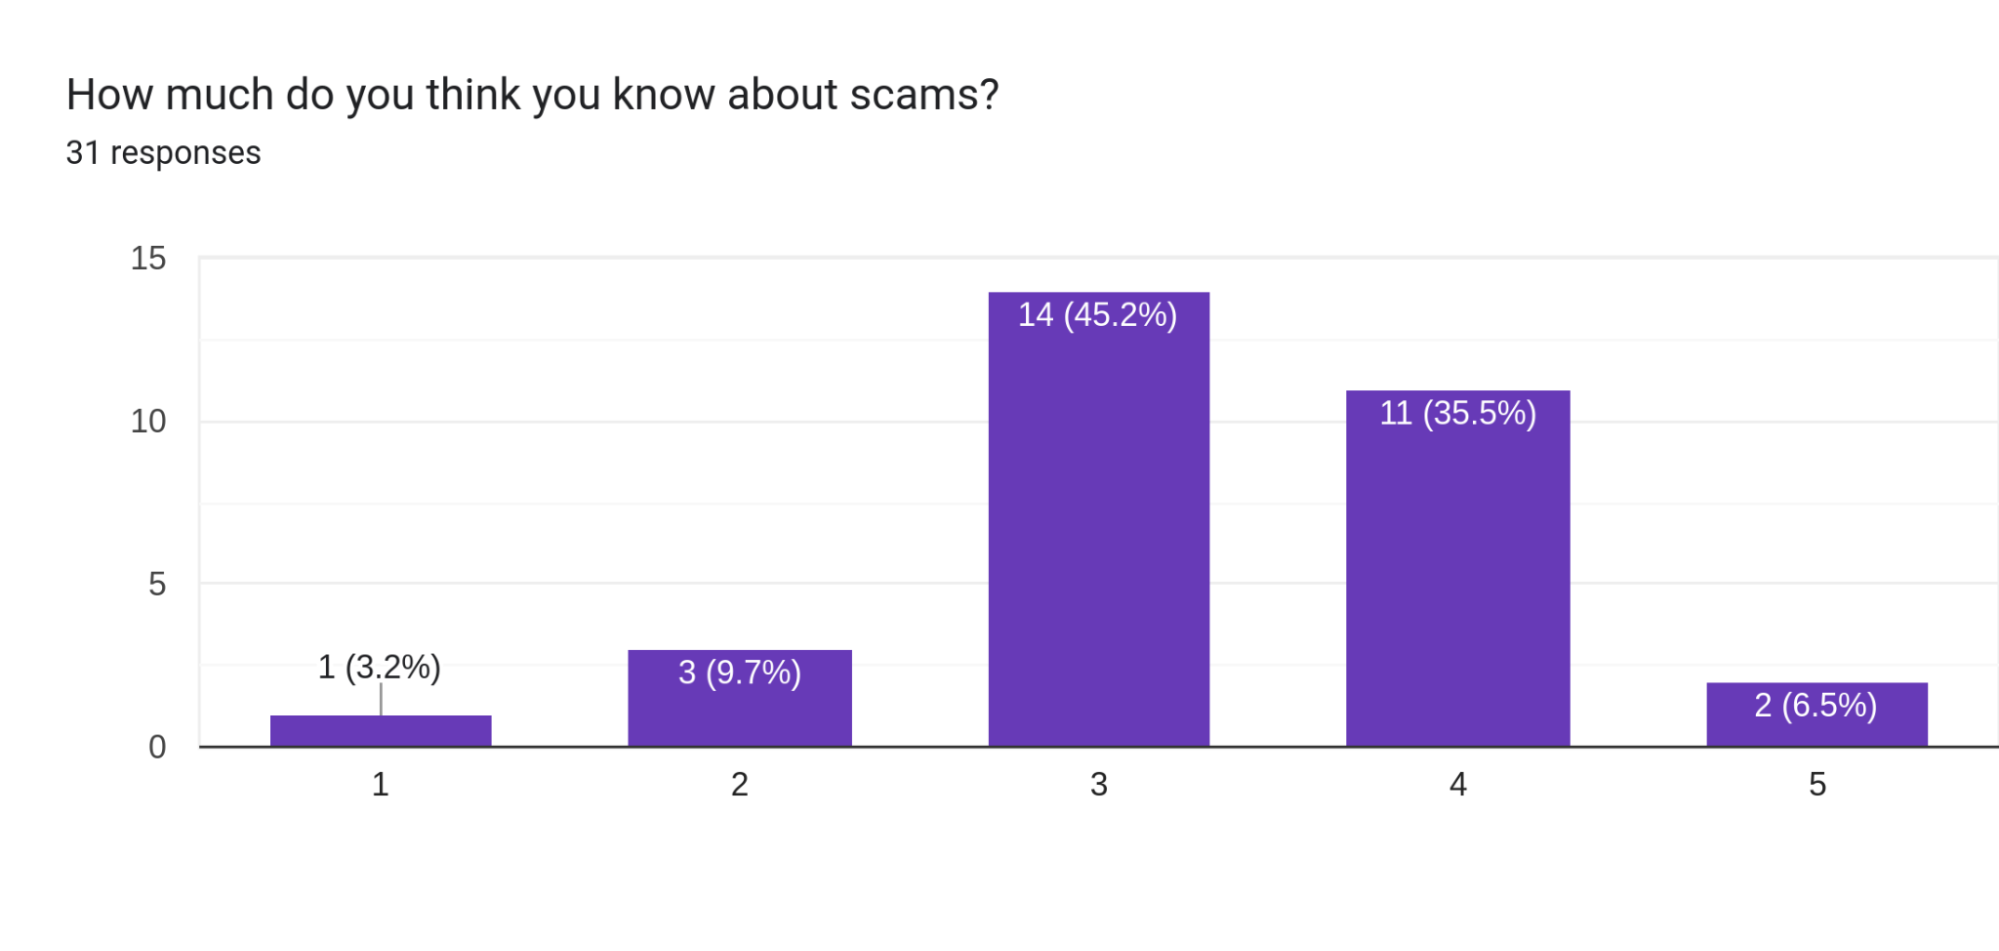
\includegraphics[width=\textwidth]{scamknowledgegraph}
  \caption{Bar chart showing majority of respondents indicating they have at
    least adequate knowledge towards scams, where 1 means ``severely
    insufficient knowledge'' and 5 means ``highly comprehensive knowledge''.
    This shows youths' complacency in their ability to identify scams; most
    think they have the minimal skills required to avoid falling prey to scams,
    but scam rates among youths suggest
    otherwise.}\label{fig:scamknowledgegraph}
\end{figure}


\subsubsection{Lack of technical knowledge}
\paragraph{} Youths are unable to recognise how common scams such as job and
investment scams work. For instance, despite initial payouts to victims (which
``[lures] them into providing more funds'') being a common scam strategy, youths
still fall for this ploy, as evidenced by job and investment scams being among
the top scams in 2022 \parencite{Hui.2023}.

\paragraph{} Additionally, scammers constantly devise new tactics, such as the
``fake friend call scam'' which has become overwhelmingly popular
\parencite{Goddard.2023}. Thus, without proactive knowledge-seeking from youth,
information on scam prevention quickly becomes irrelevant. Therefore, youth lack
the knowledge to prevent scams both in the short and long term.

\subsection{Current measures and gaps}
\subsubsection{NCPC's campaign}
\paragraph{} NCPC\footnote{National Crime Prevention Council} has launched an
anti-scam campaign with the 2023 tagline ``I Can ACT Against Scams''
\parencite{Sun.2023} and a website called ScamAlert \parencite{NCPC}.

\paragraph{} However, the campaign is intended for the general public and
therefore not tailored for youths, as suggested by the diversity of the
ambassadors of the campaign (\cref{fig:scamalert}). The underlying complacency
in youths is not addressed, as the campaign focuses on actions to take rather
than attitudes to change.

\paragraph{} Additionally, certain sections of the ScamAlert website can be
wordy, possibly resulting in low engagement with youths who tend to have a
shorter attention span \parencite{ChowHari.2022} and may be unwilling to read
the long paragraphs.

\begin{figure}[ht]
  \minipage[t]{0.45\textwidth} \centering
  
\includegraphics[width=\textwidth]{scamalert}
  \caption{Main page of the ``ACT NOW'' section on the ScamAlert website with
    representatives of varying ages, showing that it is not specifically
    targeted to our target group.}\label{fig:scamalert}
  \endminipage\hfill \minipage[t]{0.45\textwidth} \centering
  
\includegraphics[width=\textwidth]{scamalertwordy}
  \caption{Example of a wordy information page on the ScamAlert website that
    youths would be unwilling to read.}\label{fig:scamalertwordy}
  \endminipage{}
\end{figure}

\subsubsection{The Straits Times' ``STOP SCAMS'' initiative}
\paragraph{} ST's\footnote{The Straits Times} ``STOP SCAMS'' initiative features
stories of people getting scammedscam victims and advises readers on how to
avoid such scams. At the end of each article, tThe ScamAlert website is
mentioned as a resource.

\begin{figure}[ht!]
  \minipage[b]{0.45\textwidth} \centering
  
\includegraphics[width=\textwidth]{stopscams1} \endminipage\hfill
  \minipage[b]{0.45\textwidth} \centering
  
\includegraphics[width=\textwidth]{stopscams2} \endminipage{}
  \caption{Examples of “Stop Scams” features in the print version of ST, which
    is not commonly accessed by youths aged 20--29}\label{fig:stopcams}
\end{figure}

\paragraph{} While this initiative is also informative, its reach may be
limited. Only 16\% of Generation Z and 24\% of millennial readers access ST
physically \parencite{Ho.2021}. As it is inherently not guaranteed that these
scam articles reach online readers, engagement with ST’s initiative may be low.

\paragraph{} Put simply, NCPC and ST's initiatives do not consider youths'
habits and learning styles, resulting in low visibility of these resources to
youths.

\subsection{Our approach}
\paragraph{} We have a two-pronged approach:

\subsubsection{Changing attitudes}
\paragraph{} To incite behavioural change such that youth would act more
cautiously when facing scams, a mindset change is crucial
\parencite{ConnorBernal.2020}. Thus, we first need to change youths’ complacent
attitudes towards scams and ensure that they are aware that they are vulnerable
to scams.

\subsubsection{Educate}
\paragraph{} When youths are aware of the need to learn more about scams,
\emph{Educate} plugs any knowledge gaps that youths may have with regards to
identifying and avoiding scams. Even sophisticated scams have telltale
indicators which can be taught to youths, such as ``soliciting offers, asking
[for] personal information, [and the] use of hyperlinks''
\parencite{DatarColeRogers.2014}, showing that effective education can increase
their ability to identify and avoid scams.

\newpage
\subsection{Flowchart}
\begin{figure}[ht!]
  \centering 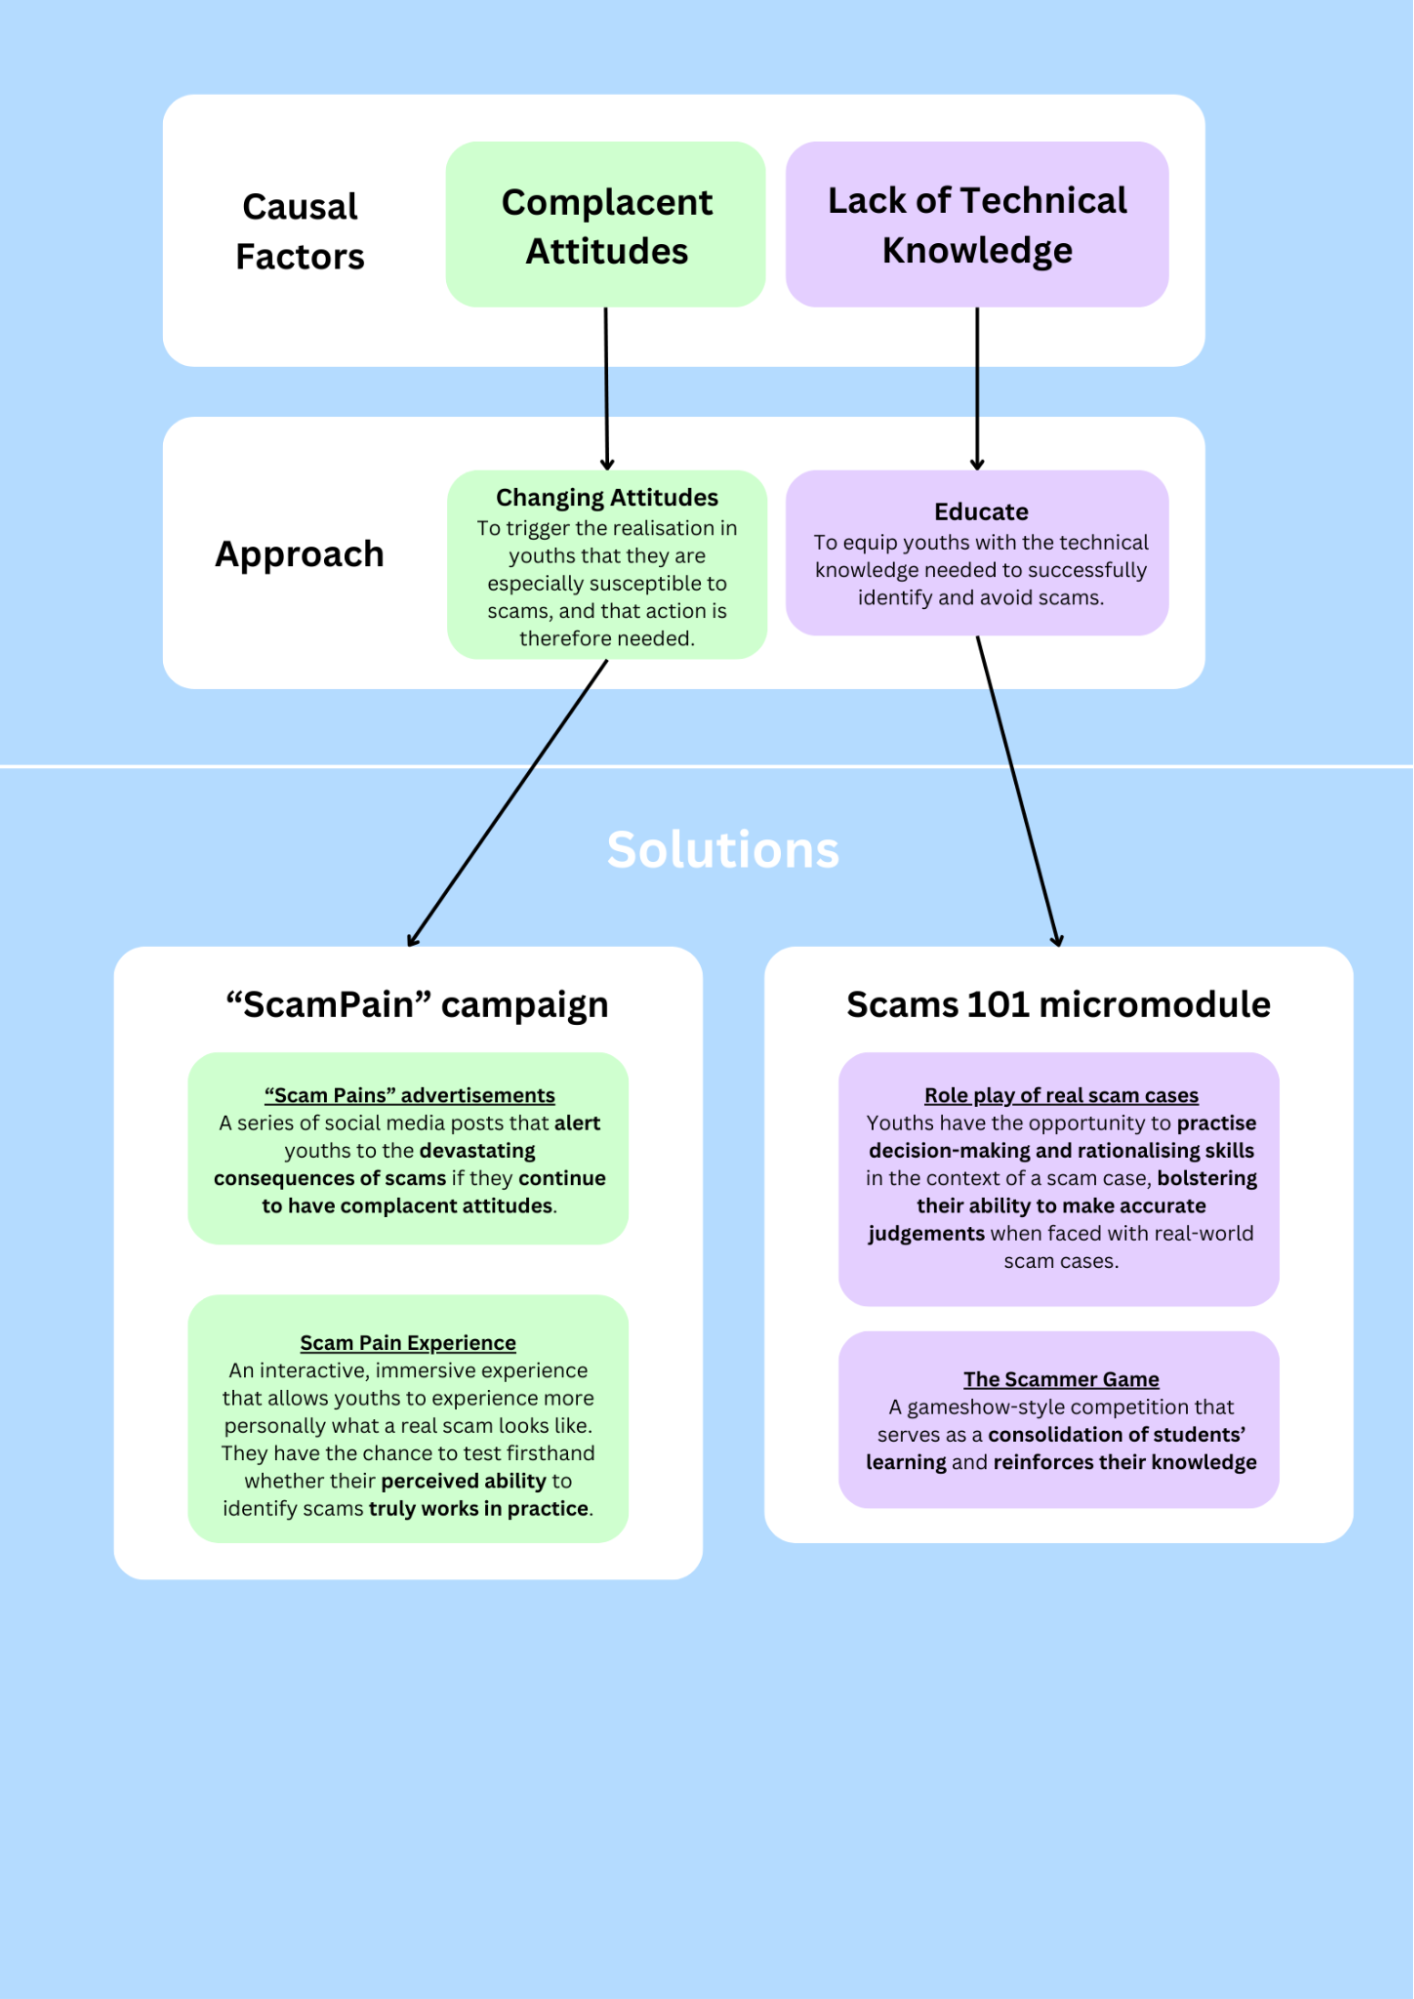
\includegraphics[width=\textwidth]{flowchart}\label{fig:flowchart}
  \caption{Flowchart overview linking our causal factors, approach and
    solutions. ``ScamPain campaign'' addresses ``Complacent Attitudes'' as the
    primary factor, while ``Scams 101 micromodule'' addresses ``Lack of
    Technical Knowledge'' as the primary factor.}
\end{figure}

\section{Changing attitudes: ``ScamPain'' campaign}
\subsection{Objectives}
\subsection{Details}
\subsubsection{Advertisments}
\subsubsection{Immersive experience}
\subsection{Evaluation}

\section{Educate: Scams 101 micromodule}
\subsection{Objectives}
\subsection{Details}
\subsection{Evaluation}

\section{Conclusion}
\subsection{Overall evaluation}
\subsection{Future development}

\newpage

\nocite{*} \printbibliography[heading=bibintoc,title={References}]

\newpage

% TC:ignore

\begin{appendices}
\end{appendices}


% TC:endignore
\end{document}
